\chapter{Conclusion and Outlook} \label{ch:cando}

The final portion of this chapter will pull all of the results and corrections together and present the final cross sections and the comparison to different theoretical models.  

\section{Systematic Uncertainties}

Systematic uncertainties arise due to our limited knowledge of the precise operating conditions and performance of the experiment and also due to any bias in our understanding of how to fundamental model the interactions.  They systematics may therefore be broken into two components: uncertainties to the jet energy scale (JES) which shifts the momentum spectra along the x-axis and uncertainties in the jet yield which shift the spectra along the y-axis.  The systematical and statistical uncertainties presented in this analysis will be presented as errors to the yield of the spectra.  Due to the fact that the $p_{T}$ distribution follows a power law function, $dN/dp_{T} \sim p_{T}^{-5}$ uncertainties in the JES are converted to yield uncertainties by dividing each one by 5.
Due to the low statistics at the highest $p_{T}$ bins in this analysis, uncertainties in this regime my have large statistical fluctuations.  Small ,systematic variations for the input of the jet spectra will have a dramatic effect over sparsely filled bins versus bins with a low granularity.  As such it may be necessary to extrapolate the systematic from a low $p_{T}$ bin to those at the highest $p_{T}$ range.  The systematic were performed on both the MB and EMCal triggered data samples but no large variation was observed between the two, thus only the uncertainties from the MB sample are shown and are extrapolated to the triggered data.


\subsection{Systematic Uncertainty to Jet Energy Scale}

The following sections present and discuss the uncertainties cause by shifts to the JES.

\subsubsection{Tracking Efficiency Sensativity}
Only a fraction of charged tracks generated by the hard scattering of two protons will be detected in the TPC due to finite track efficiency.  Uncertainties in the efficency of the TPC were studied and found to account for a 5\% discrepancy\cite{Abelev:2013ala}.  Reproducing this efficency was performed by randomly throwing out 5\% of the tracks from each event from the 8 TeV data samples and remeasuring the jet spectra.  All of the inputs for jet finding were maintained.


\begin{figure*}[t!]
$\begin{array}{rl}
    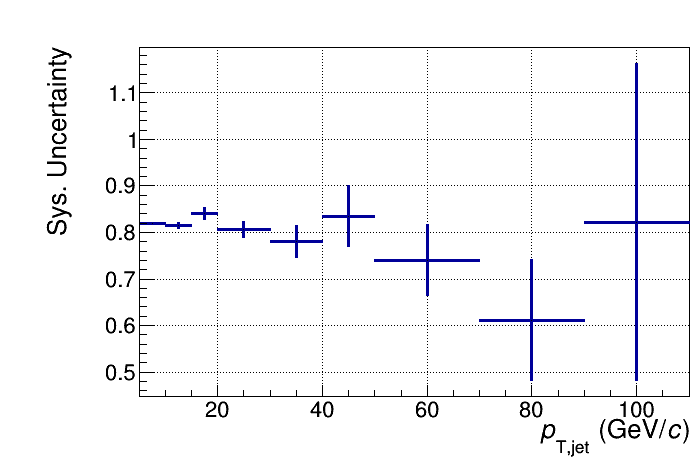
\includegraphics[width=0.40\textwidth]{SysR02_TrkEff} &
    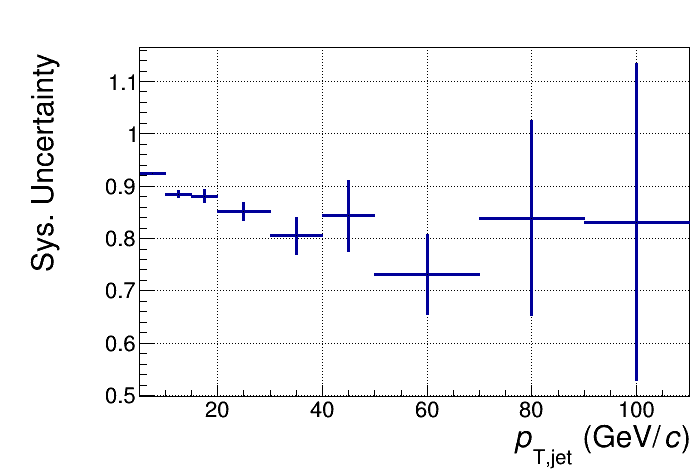
\includegraphics[width=0.40\textwidth]{SysR03_TrkEff}\\
    \multicolumn{2}{c}{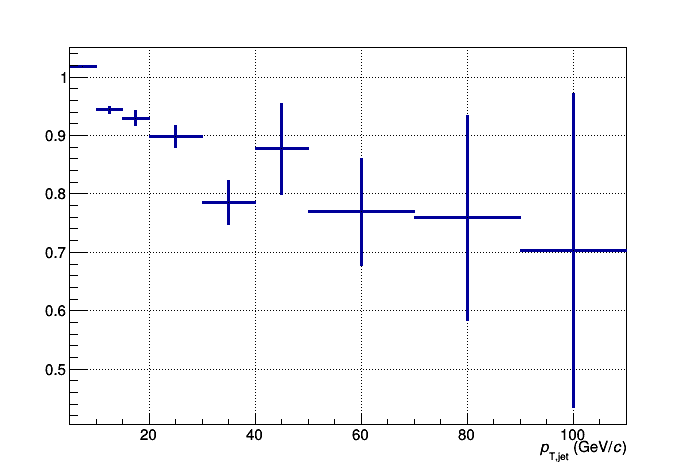
\includegraphics[width=0.40\textwidth]{SysR04_TrkEff}}
\end{array}$
\caption[Systematic due to TPC tracking efficiency.]{\label{fig:trkeff}Systematic due to TPC tracking efficiency; R = 0.2 \textit{(top left)}, R = 0.3 \textit{(top right)}, R = 0.4 \textit{(bottom)}.}
\end{figure*}

\noindent
Figure \ref{fig:trkeff} shows the systematical uncertainties for R = 0.2 (top left), R = 0.3 (top right), and R = 0.4 (bottom) jets.  A 10\% systematic was applied to R = 0.2 and R = 0.3 jets while a 15\% systematic uncertainty was given to R = 0.4 jets for this analysis.

\subsubsection{Hadronic Correction Systematic}

\begin{figure*}[t!]
$\begin{array}{rl}
    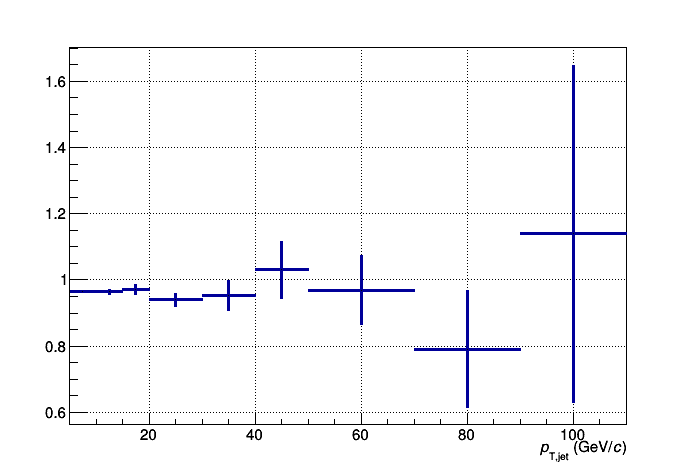
\includegraphics[width=0.40\textwidth]{SysR02_F07} &
    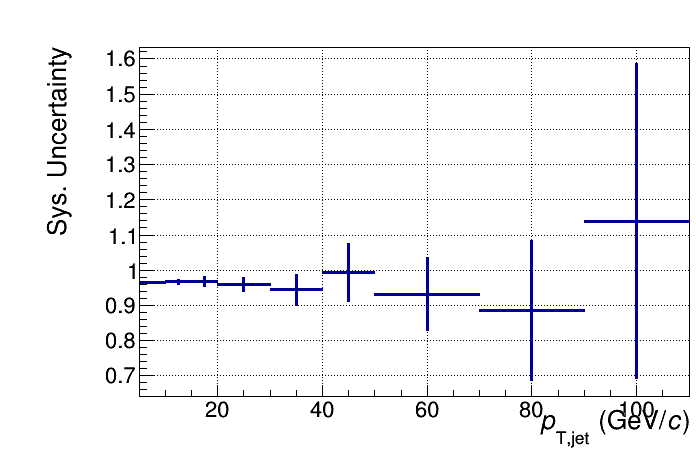
\includegraphics[width=0.40\textwidth]{SysR03_F07}\\
    \multicolumn{2}{c}{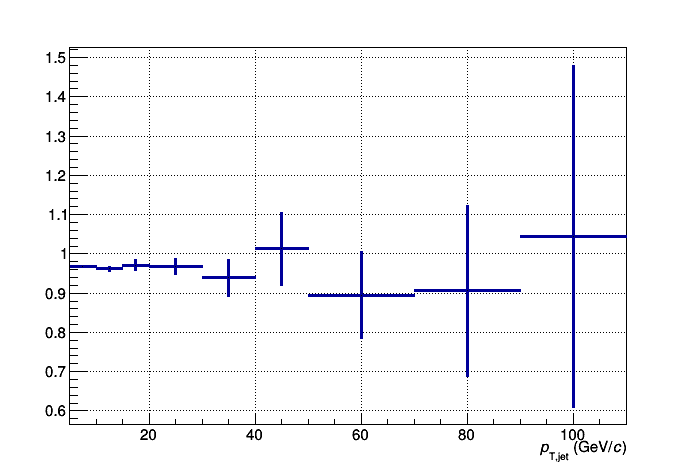
\includegraphics[width=0.40\textwidth]{SysR04_F07}}
\end{array}$
\caption[Systematic due to Hadronic correction.]{\label{fig:hadeff}Systematic due to hadronic correction efficiency; R = 0.2 \textit{(top left)}, R = 0.3 \textit{(top right)}, R = 0.4 \textit{(bottom)}.}
\end{figure*}

\subsubsection{Sensativity to EMCal Clusterization Algorithm}
As previously stated, the clusterizer used in this thesis was the v2 algorithm. This algorithm was used in both the detector-level Monte Carlo and data analysis.  In order to test the sensitivity the JES has to the clusterization algorithm a different algorithm was chosen and a new spectra was generated.  The v1 algorithm was choosen and is similar to the v2 algorithm with the exception that the total size of the cluster is forced to be smaller then nine towers.  Similar to the other systematic presented we see a large anti-correlated bin-to-bin variatiaions at high-$p_{T}$ due to sparsely field binning.  

\begin{figure*}[t!]
$\begin{array}{rl}
    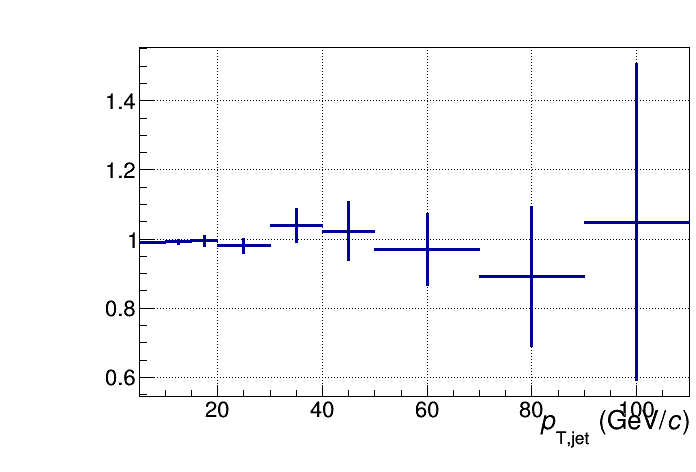
\includegraphics[width=0.40\textwidth]{SysR02_v1Clusterization} &
    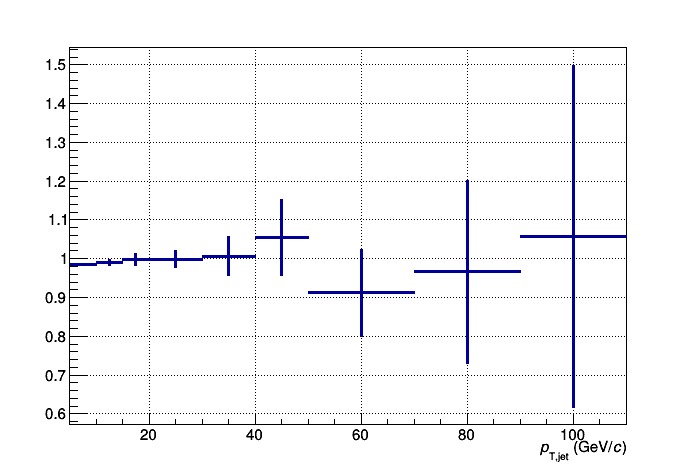
\includegraphics[width=0.40\textwidth]{SysR03_v1Clusterization}\\
    \multicolumn{2}{c}{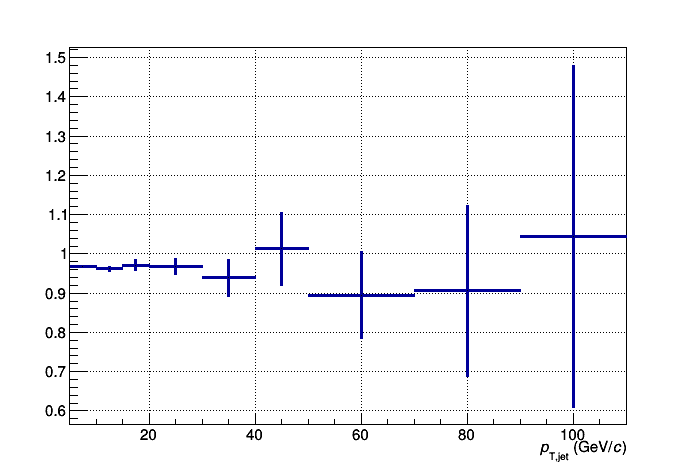
\includegraphics[width=0.40\textwidth]{SysR04_F07}}
\end{array}$
\caption[Systematic due to clusterization algorithm.]{\label{fig:cluseff}Systematic due to EMCal clusterization algorithm; R = 0.2 \textit{(top left)}, R = 0.3 \textit{(top right)}, R = 0.4 \textit{(bottom)}.}
\end{figure*}

\subsection{Systematic Uncertainty to Jet Yield}
The following sections discuss the systematic uncertainties affecting the jet yield.

\subsubsection{Track $p_{T}$ resolution}
The momentum resolution of TPC is estimated using the covariance matrix, Figure\ref{fig:trackpcovmatrix}, generated from a Kalman filtering\cite{Fruhwirth:1987fm} pad signal on the TPC read-out region.  To estimate the systematic due to the $p_{T}$ resolution tracks are smeared 

\begin{figure}[h]
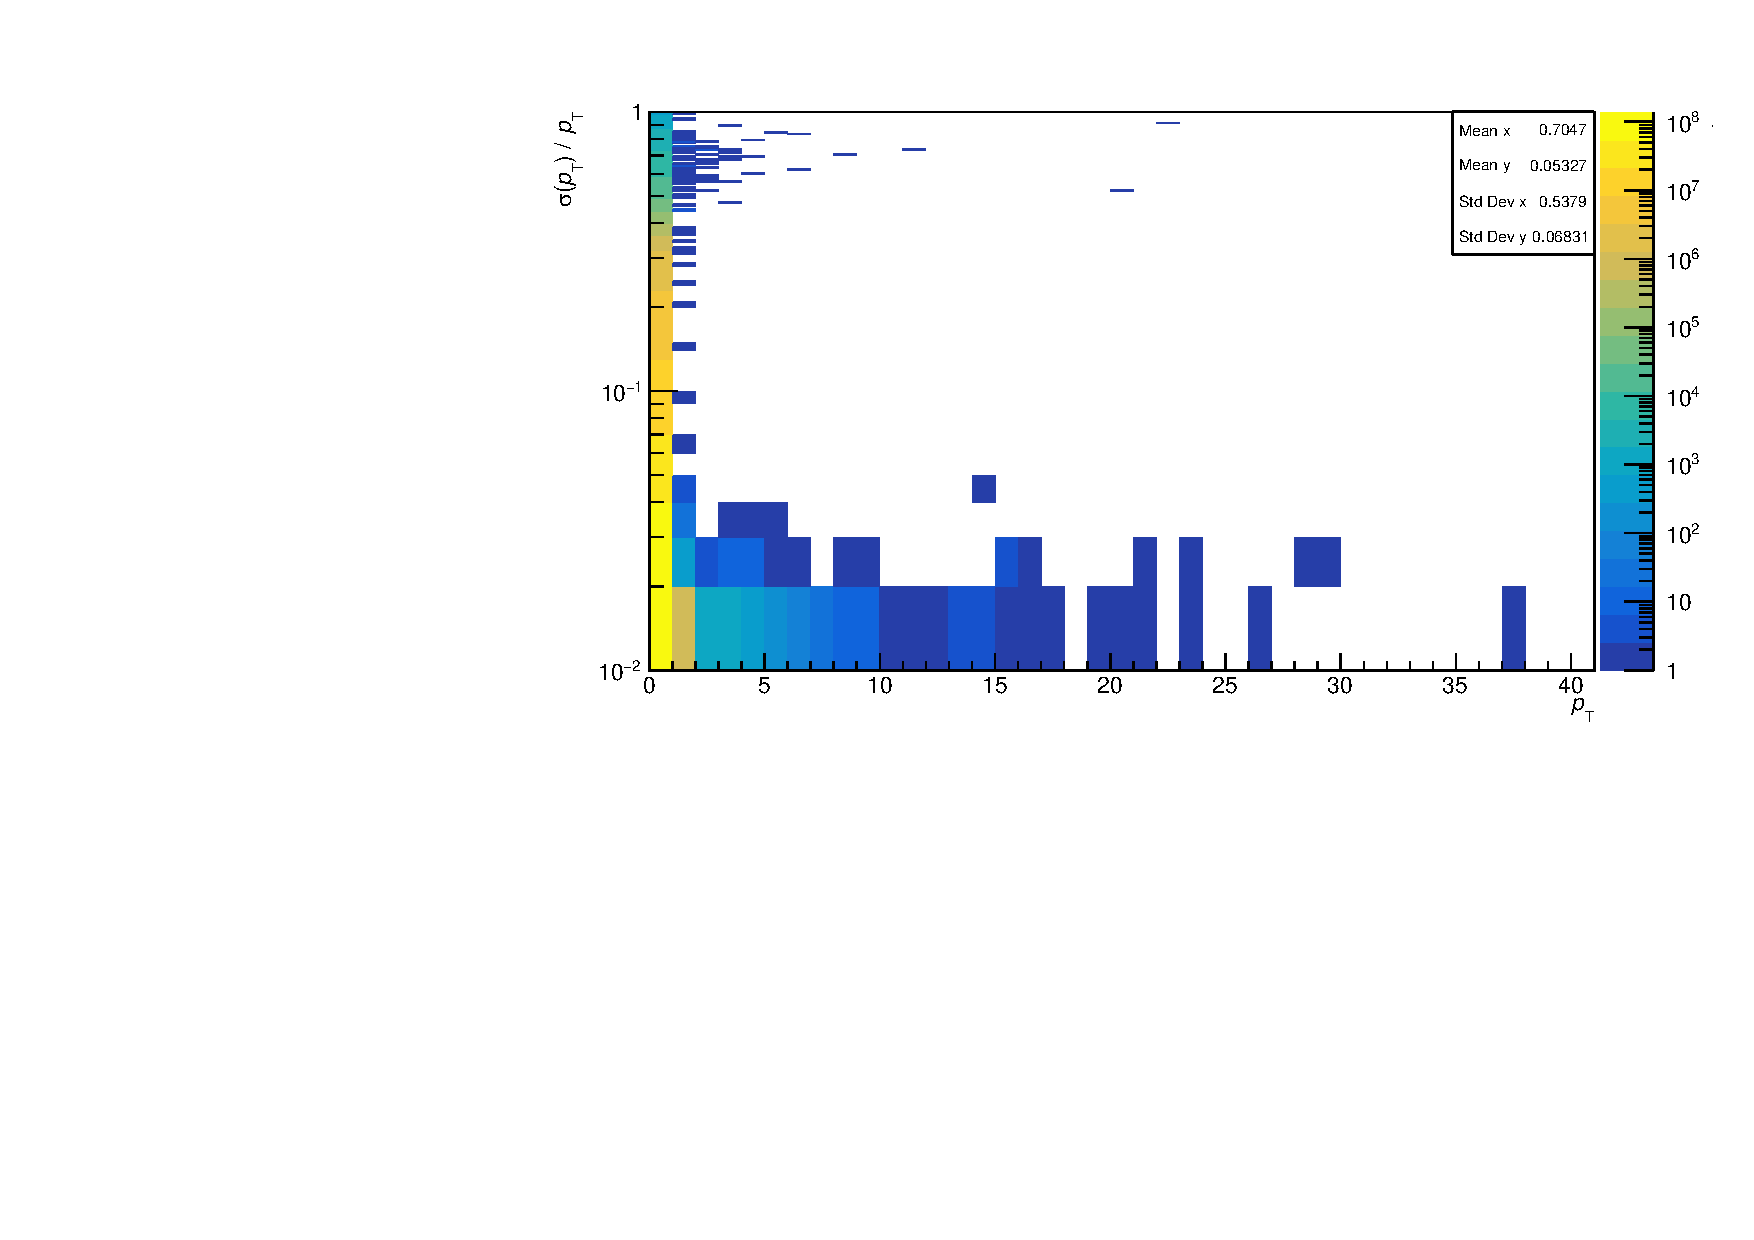
\includegraphics[width=8cm]{trackcovmatrix}
\centering
\caption{Inclusive track resolution, Min Bias 8 TeV.}
\label{fig:trackpcovmatrix}
\end{figure}

Most tracks have below 1\% momentum resolution and the tracks with $\sigma(p_{T})/p_{T} \geq$ 1\% tend to be tracks below 200 MeV tracks.  To measure the $p_{T}$ resolution I smeared each track from the Min Bias data by a Gaussian function which would alter the track $p_{T}$ by up to 1\% of its original value and remeasure the spectra.  

\begin{figure*}[t!]
$\begin{array}{rl}
    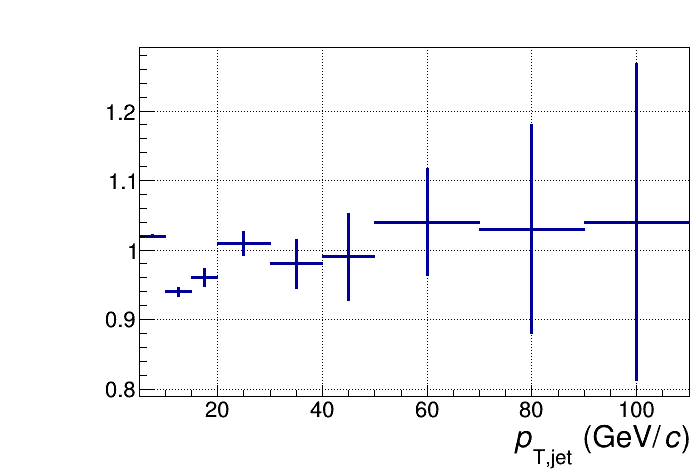
\includegraphics[width=0.40\textwidth]{SysR02_PtReso} &
    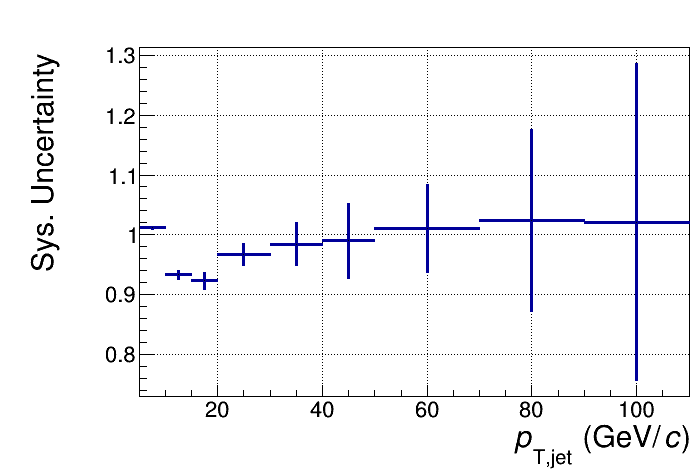
\includegraphics[width=0.40\textwidth]{SysR03_PtReso}\\
    \multicolumn{2}{c}{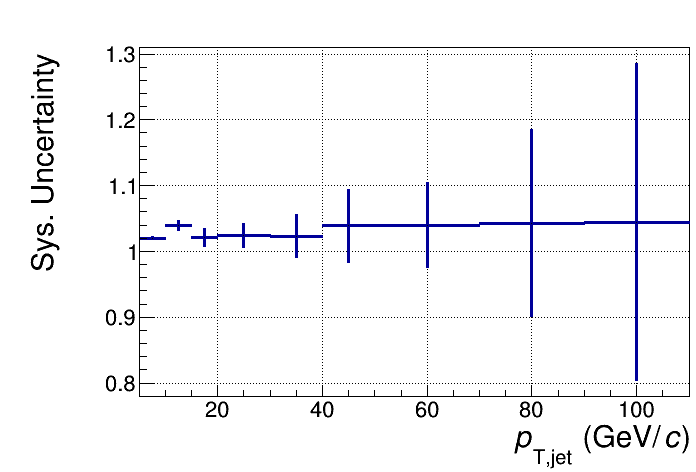
\includegraphics[width=0.40\textwidth]{SysR04_PtReso}}
\end{array}$
\caption[Systematic due to $P_{T}$ resolution.]{\label{fig:pTeff}$P_{T}$ resolution; R = 0.2 \textit{(top left)}, R = 0.3 \textit{(top right)}, R = 0.4 \textit{(bottom)}.}
\end{figure*}


\subsubsection{Cluster Energy resolution}

\begin{figure*}[t!]
$\begin{array}{rl}
    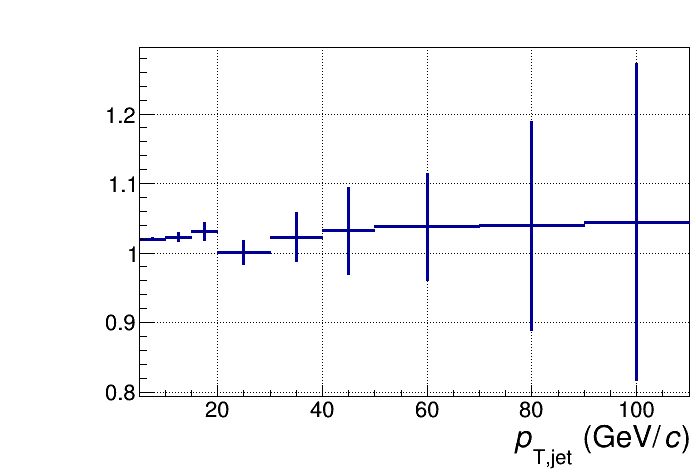
\includegraphics[width=0.40\textwidth]{SysR02_EReso} &
    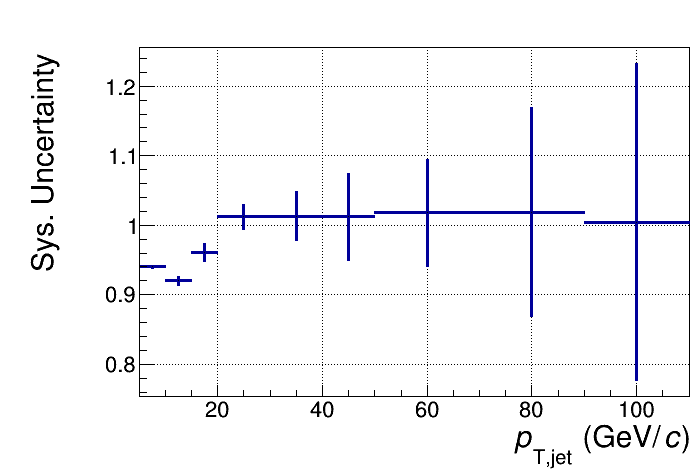
\includegraphics[width=0.40\textwidth]{SysR03_EReso}\\
    \multicolumn{2}{c}{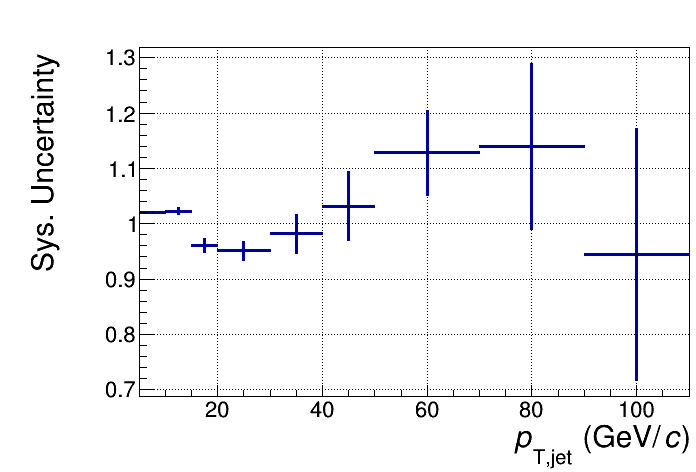
\includegraphics[width=0.40\textwidth]{SysR04_EReso}}
\end{array}$
\caption[Systematic due to energy resolution.]{\label{fig:pTeff}energy resolution; R = 0.2 \textit{(top left)}, R = 0.3 \textit{(top right)}, R = 0.4 \textit{(bottom)}.}
\end{figure*}

\subsubsection{Min Bias Luminosity and Uncertainty}

The luminosity of a hadronic collider, $\mathscr{L}$, is given by the expression



\begin{equation}
\mathscr{L} = \frac{R}{\sigma}
\label{eq:xlumdef}
\end{equation}

\noindent
where R is the interaction rate and $\sigma$ is the visible cross section.  Due to the fact that we only measure events within a 10 cm window within the primary vertex region we must scale the total luminosity to that which is delievered within the primary vertex region of the ALICE experiment.  This scale factor is determined by dividing the total number of MB events to those accepted within the 10 cm window.  $N^{tot}_{MB} / N^{10 cm vertex}_{MB}$ = 1.024 from the acceptance criteria held in this analysis.
The luminosity along with its uncertainty were determined during a a special Van der Meer scan run in April of 2012\cite{ALICE-PUBLIC-2017-002}.  The total systematic uncertainty for the minimum bias (MB) trigger were obtained by measuring the visible cross section using the T0 and V0 detectors.  The MB trigger was defined as V0AND which required a hit in both tjhe V0A and V0C.  The cross section was reported as being a combined average for MB with the V0AND as, 

\begin{equation}
\sigma_{V0} = (55.8 \pm 1.2) mb
\label{eq:xlumdef}
\end{equation}

\noindent
with a combined systematic uncertainty of 2.19\% on the visible cross section and 2.60\% on the luminosity. 


\subsubsection{Total Uncertainty}

A summary of the total systematic errors used in the final analysis.

\begin{tabular}{ |p{5cm}||p{3cm}|p{3cm}|p{3cm}|  }
 \hline
 \multicolumn{4}{|c|}{Systematic Errors} \\
 \hline
 Systematic &R = 0.2 Jets & R = 0.3 Jets& R = 0.4 Jets\\
 \hline
Clusterization (low-$p_{T}$) & 1.0\%    &1.0\%&  3.0\%\\
 (high-$p_{T}$)           &  5.0\%  & 10.0\%   &  10.0\%\\
Hadronic (all bins)&   5.0\% & 4.0\% & 5.0\%\\
Track Eff (low-$p_{T}$)&20.0\% & 15.0\% & 15.0\%\\
 (high-$p_{T}$)            &  25.0\%  & 20.0\%   &  25.0\%\\
Unfolding (all bins)& 6.0\% & 6.0\%&  6.0\%\\
$p_{T}$ Resolution & 2.0\% & 1.0\% & 4.0\%\\
E Resolution& 2.0\%   &1.0\% & 5.0\%\\
Luminosity (all bins) & 2.2\%  & 2.2 \% & 2.2\%\\
 \hline
 \hline
Total Sys (low-$p_{T}$) & 8.9\%  & 6.6\% & 10.9\%\\
(high-$p_{T}$) & 10.3\%  & 9.1 \% & 14.5\%\\
\hline
\end{tabular}


\noindent

The systematics from the yield and JES are added in quadrater together and this is combined in quardrater with the statistical errors.

\section{8 TeV Inclusive Jet Results from CMS and ATLAS}

CMS\cite{CMS:2013kda} and ATLAS\cite{Aaboud:2017dvo} both reported the double differential cross section for inclusive jets at 8 TeV.  

\begin{figure}[h]
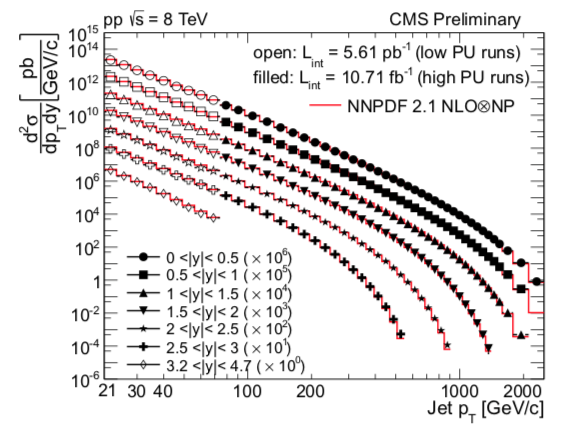
\includegraphics[width=10.0cm]{CMS8TeVJet}
\centering
\caption{8 TeV CMS inclusive jet cross sections with radii of R = 0.7 and binned by jet rapidity compared to NLO calculations with non-pertubative corrections\cite{CMS:2013kda}.}
\label{fig:CMS8TeVRescale}
\end{figure}

\begin{figure}[h]
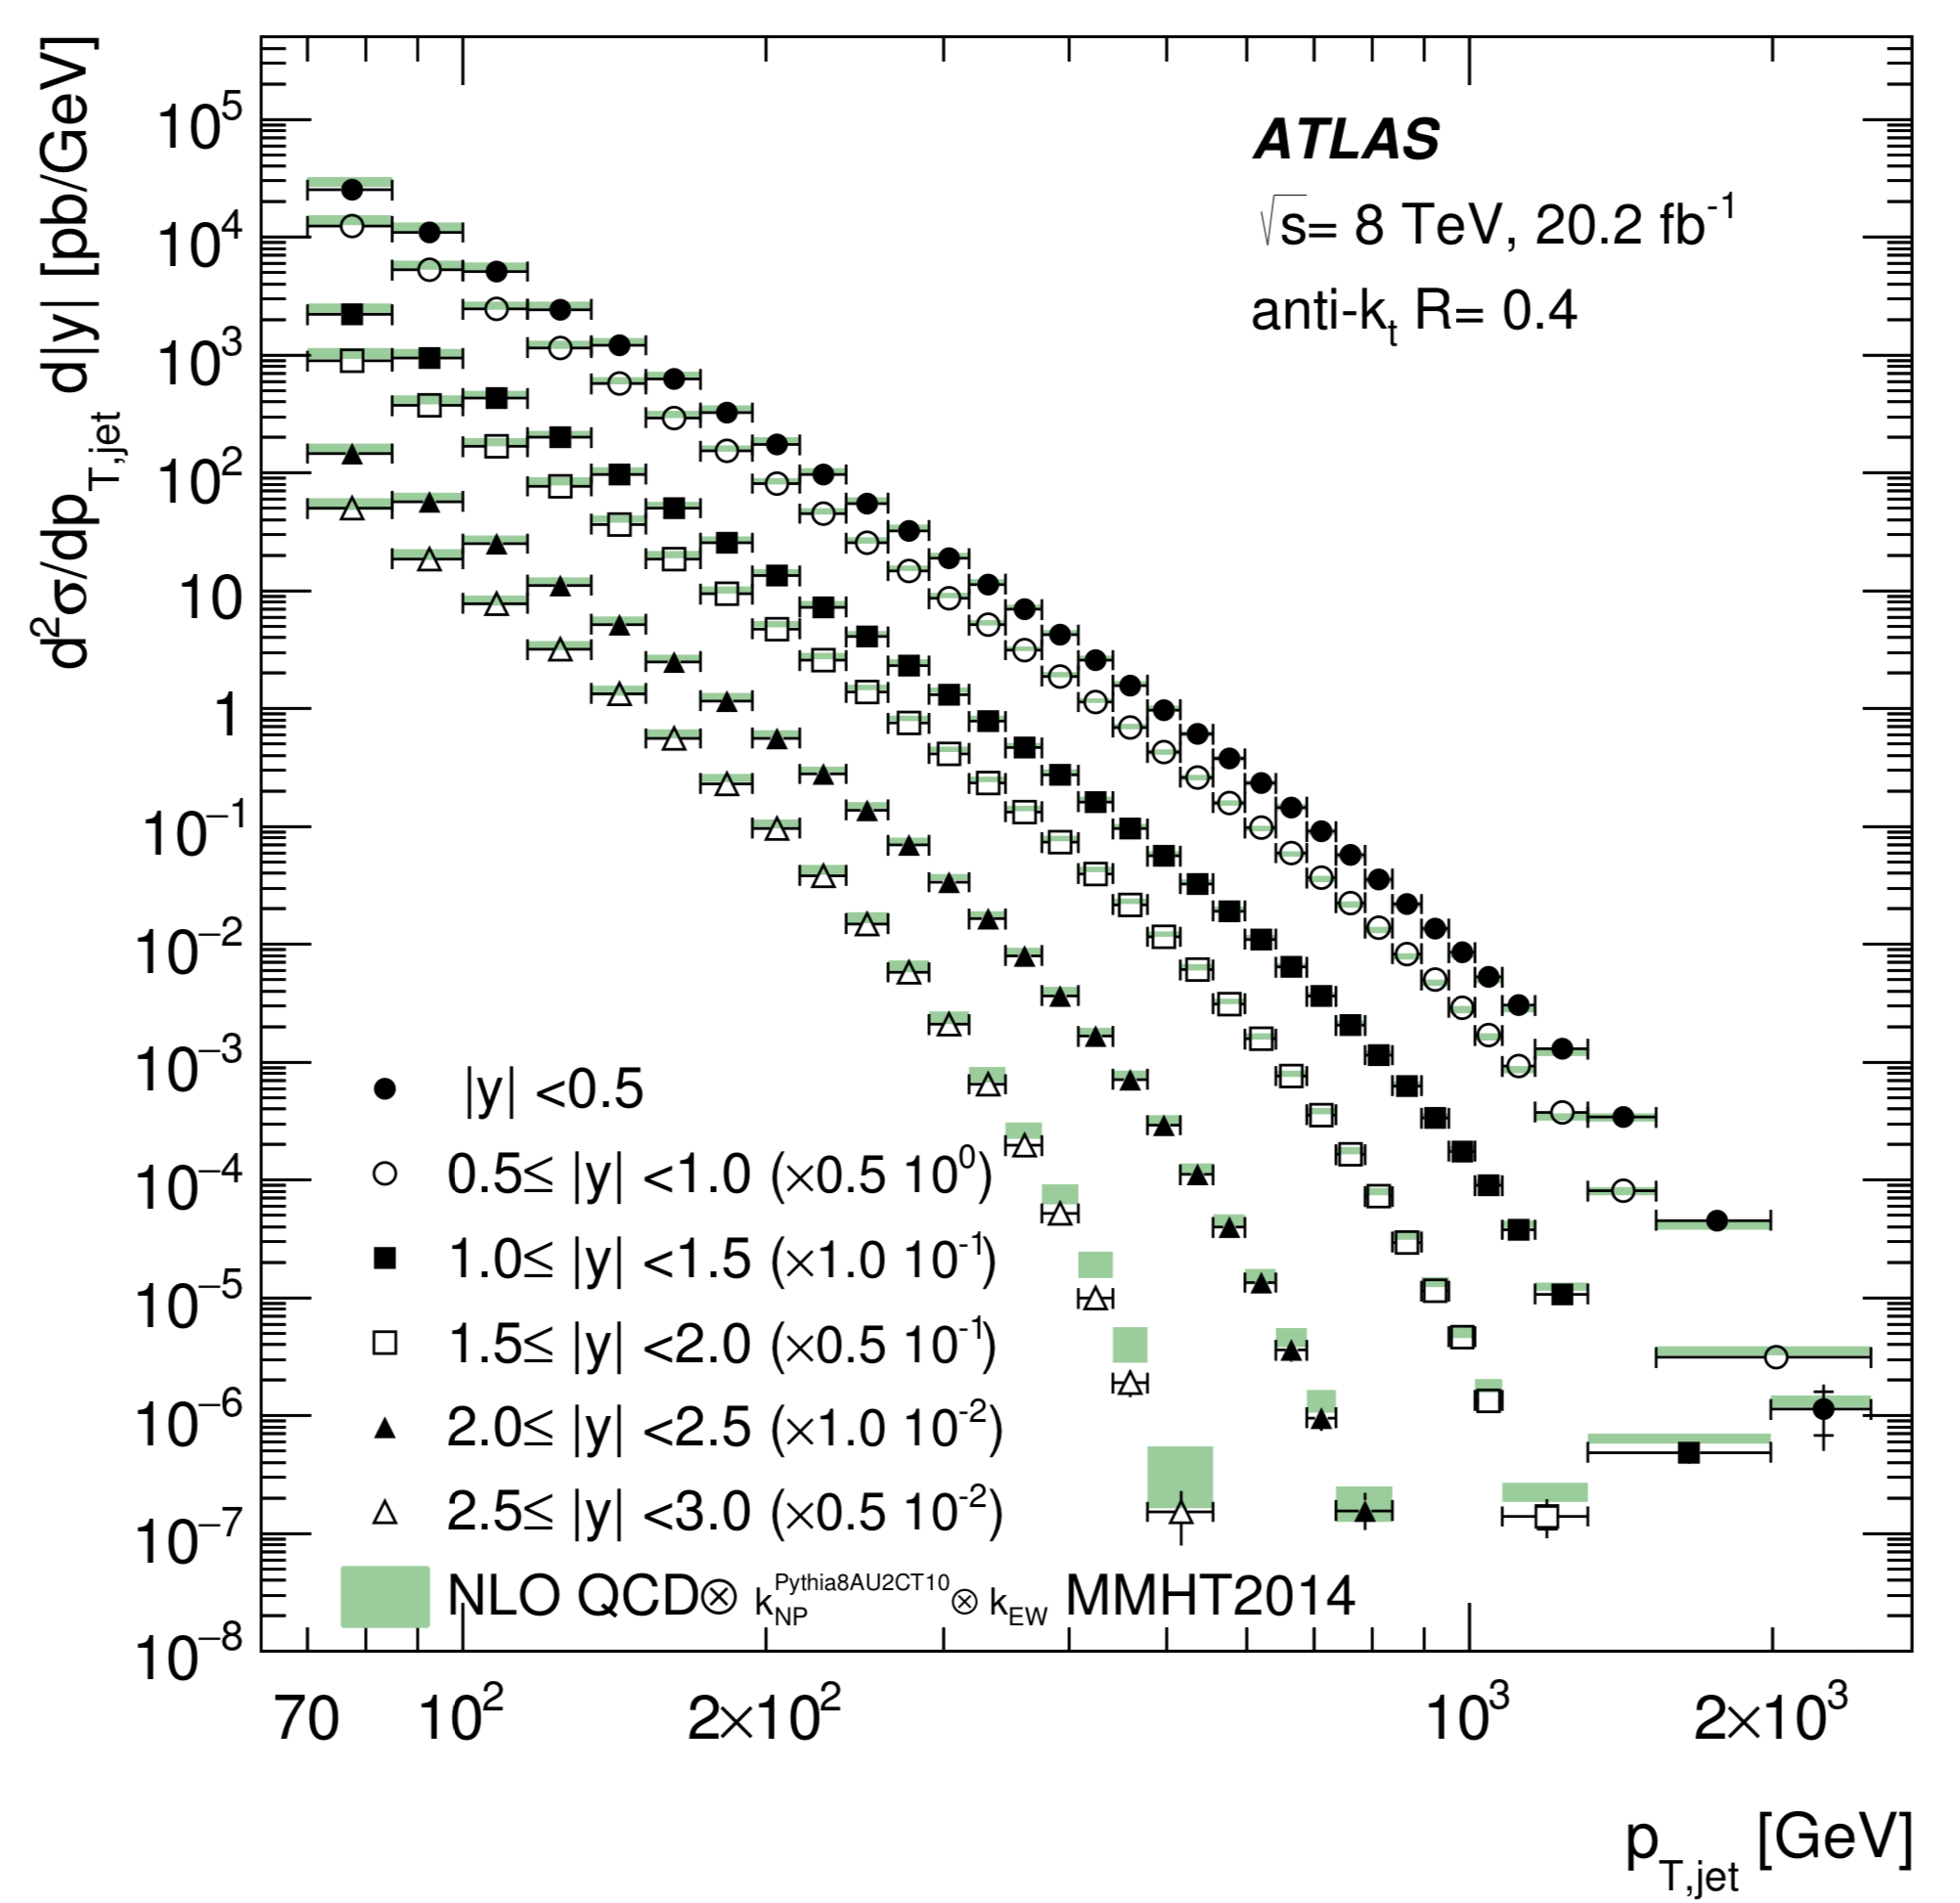
\includegraphics[width=10.0cm]{ATLAS8TeVJet}
\centering
\caption{R = 0.4 inclusive jet cross section at 8 TeV from ATLAS in binned by jet rapidity compared to NLO QCD predictions\cite{Aaboud:2017dvo}.}
\label{fig:ATLAS8TeV}
\end{figure}

\begin{figure}[h]
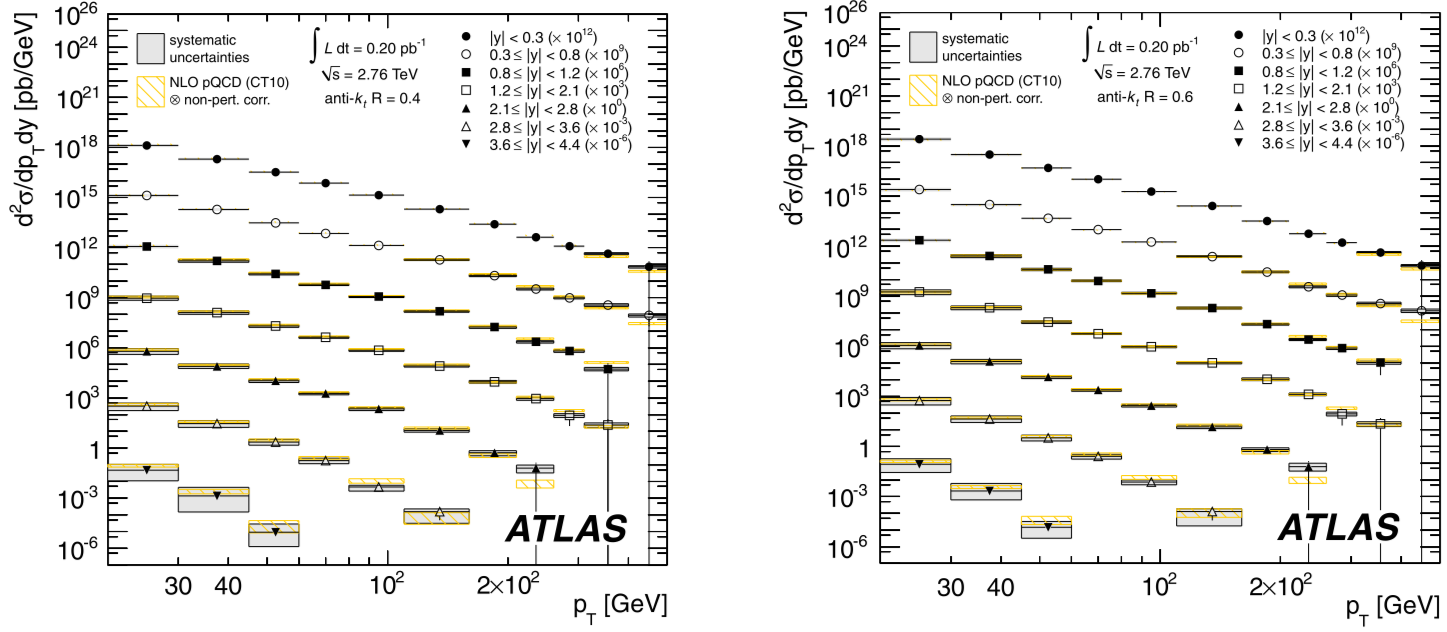
\includegraphics[width=14.0cm]{ATLAS8TeVJetRecaled}
\centering
\caption{The 8 TeV ATLAS jet cross sections rescaled to better show comparissons with NLO and non-pertubative calculations at low $p_{T}$\cite{Aaboud:2017dvo}.}
\label{fig:ATLAS8TeVRescale}
\end{figure}

\section{Inclusive Jet Spectra and Cross Section Ratios at 2.76 TeV}
Inclusive jet spectra and cross section ratios were measured in the ALICE experiment using a 2011 pp 2.76 TeV data sample\cite{MA2013319}.  Jets were reconstructed using TPC tracks and EMCal clusters with the FastJet Anti-$K_{T}$ algorithm.  Tracks with a minimum $p_{T} \geq \,$ 150 MeV and constrained to within 10 cm of the primary vertex were accepted into the jet finder.  EMCal clusters were 

\begin{figure}[h]
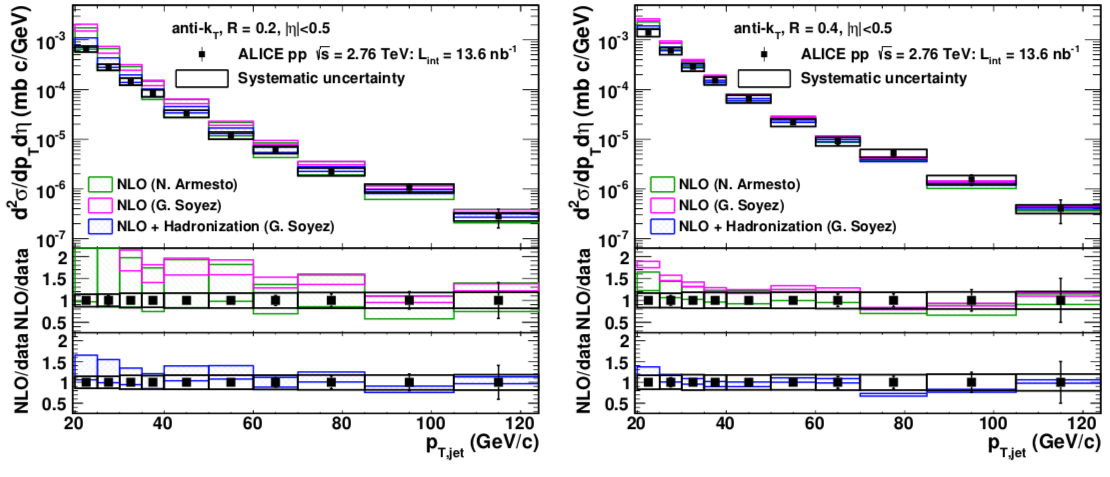
\includegraphics[width=17cm]{AliceppRongRong}
\centering
\caption{Inclusive differential cross section from the 2.76 TeV proton proton run with ALICE}
\label{fig:RunEff}
\end{figure}

\begin{figure}[h]
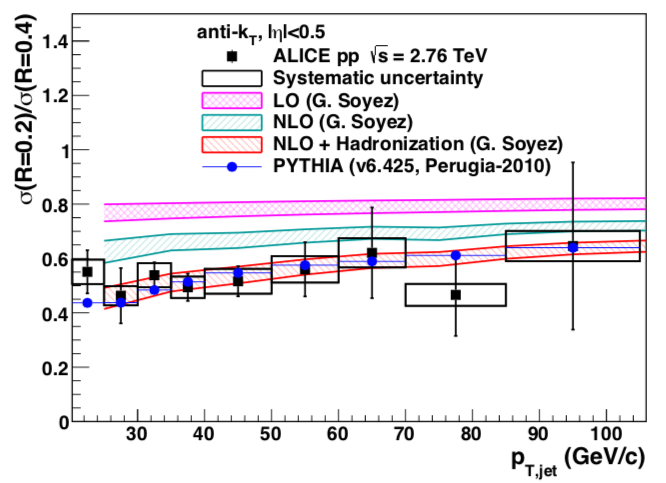
\includegraphics[width=10cm]{AliceRatioRongRong}
\centering
\caption{LHC state during the 8 TeV run. }
\label{fig:RunEff}
\end{figure}

\begin{figure}[!tbp]
  \centering
  \begin{minipage}[b]{0.4\textwidth}
    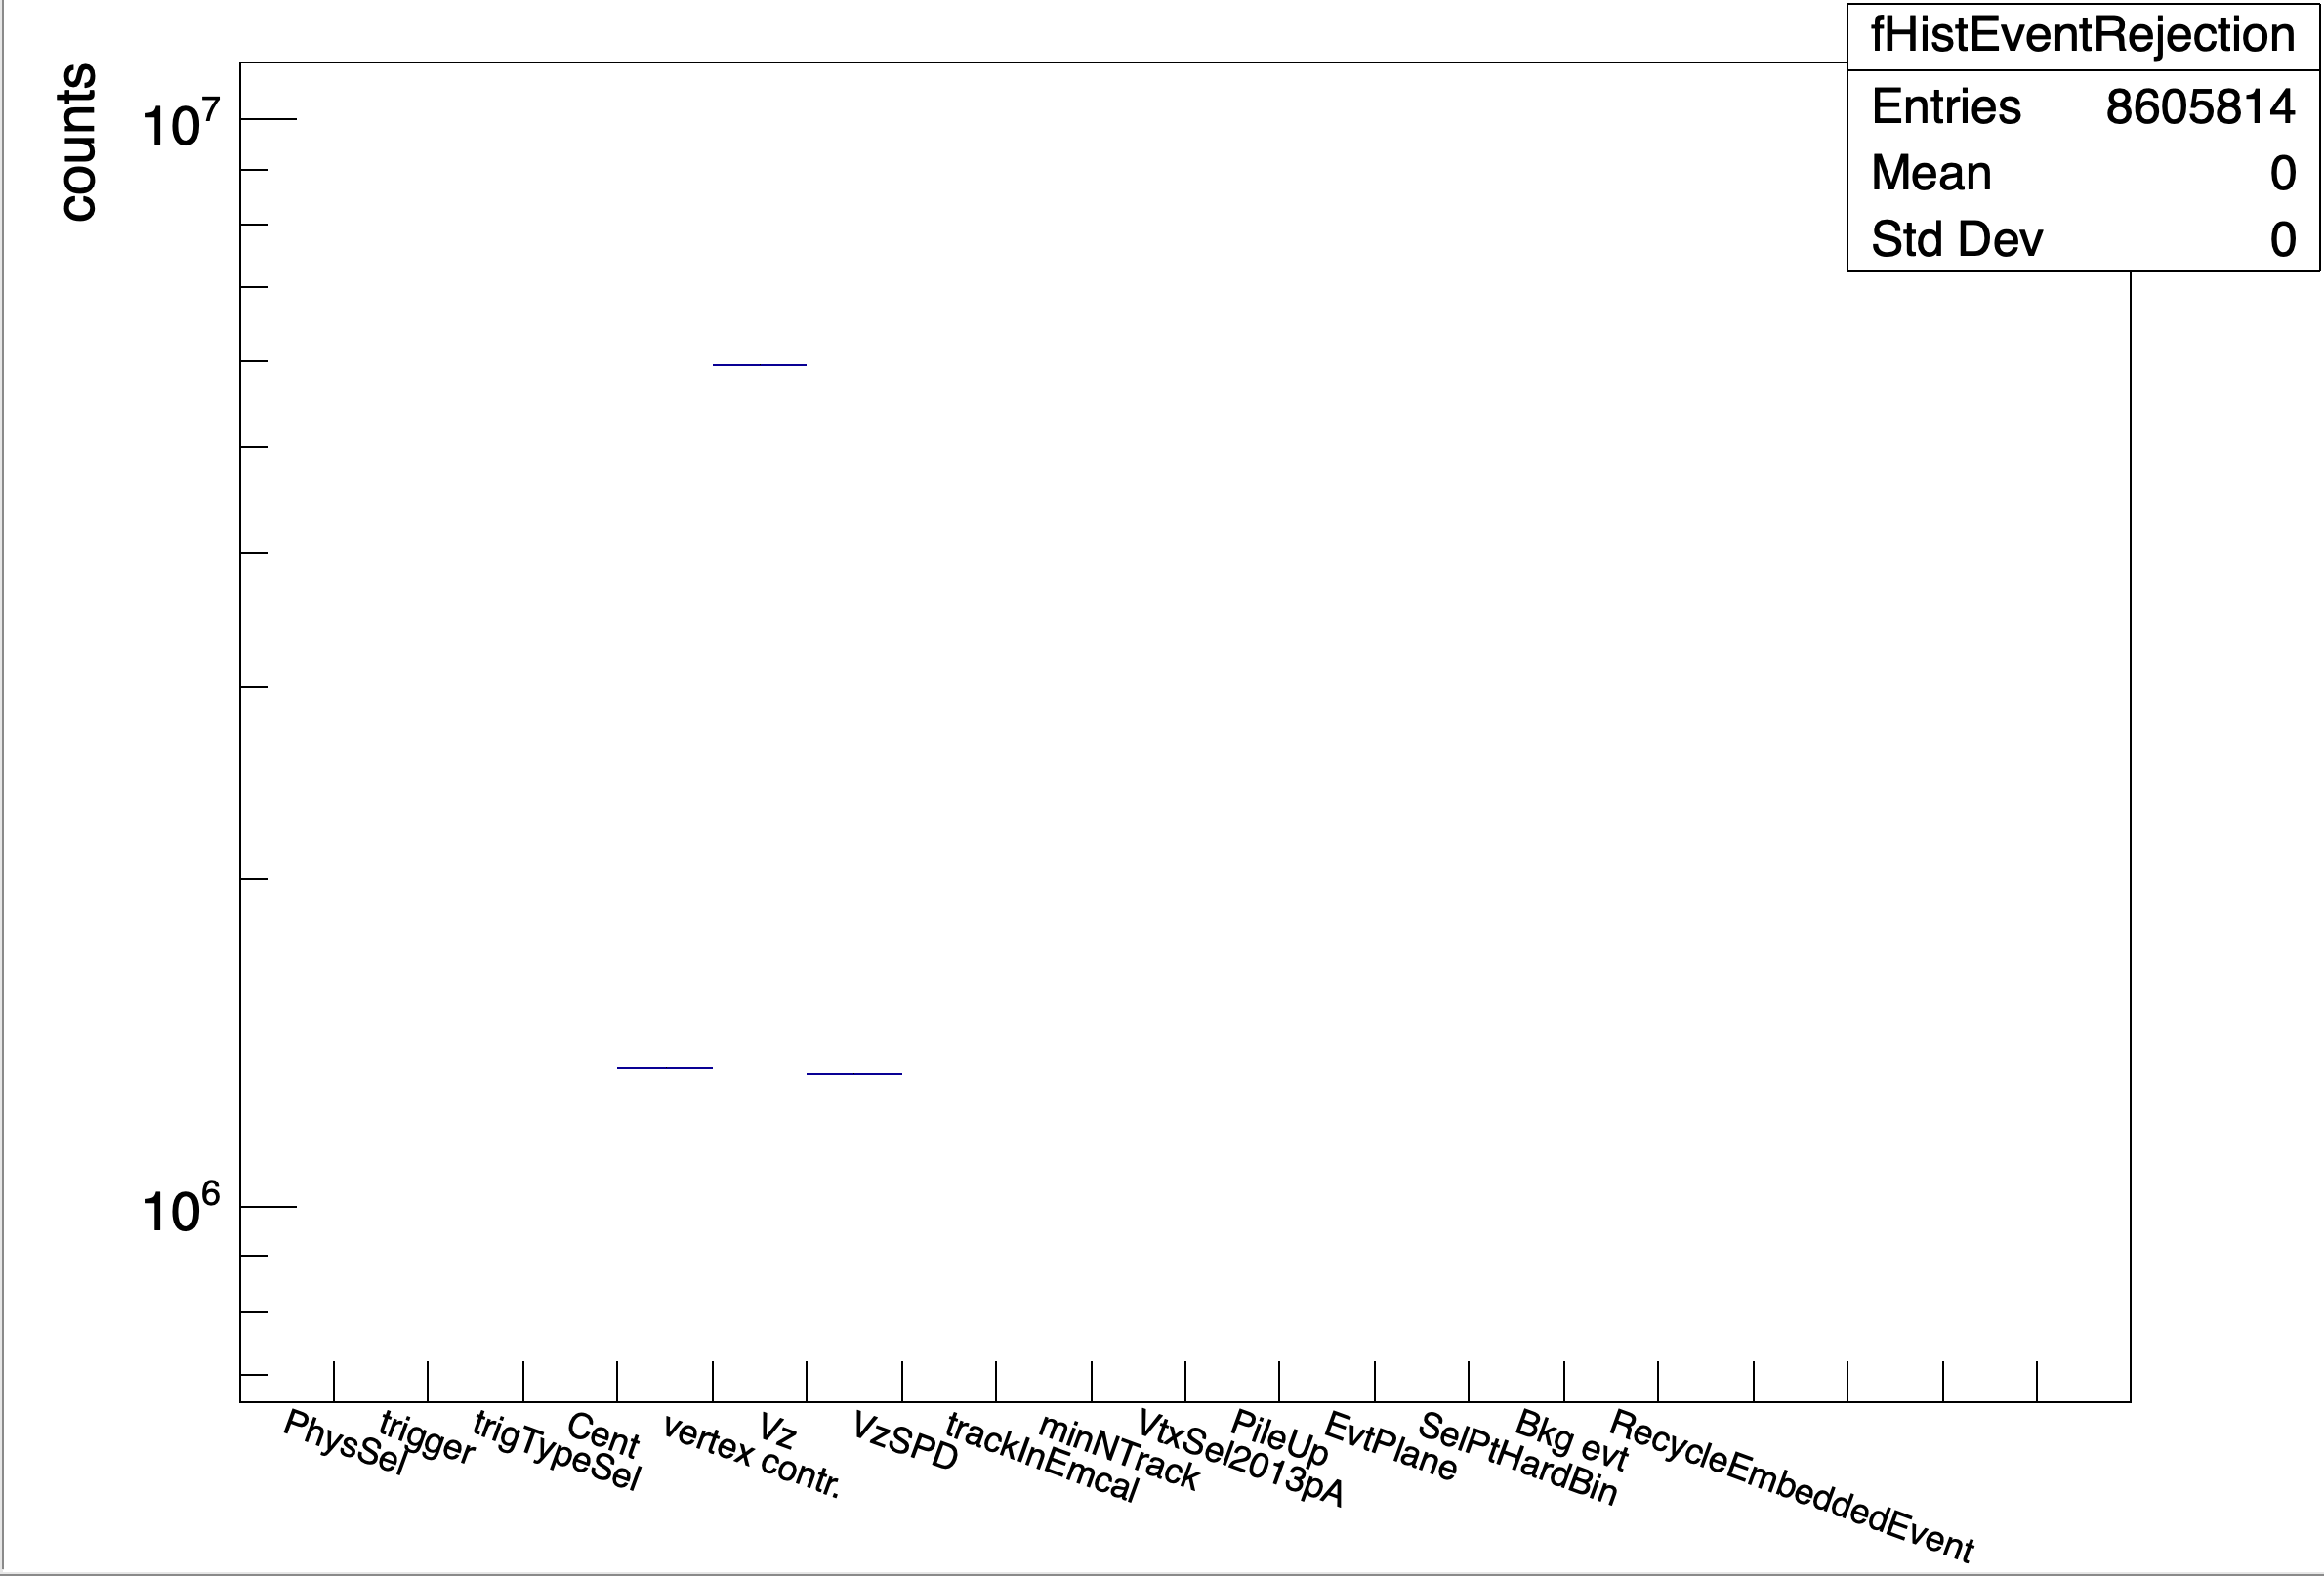
\includegraphics[width=\textwidth]{EventRejectionMB}
    \caption{Mimimmum Bias Event Rejection}
  \end{minipage}
  \hfill
  \begin{minipage}[b]{0.49\textwidth}
    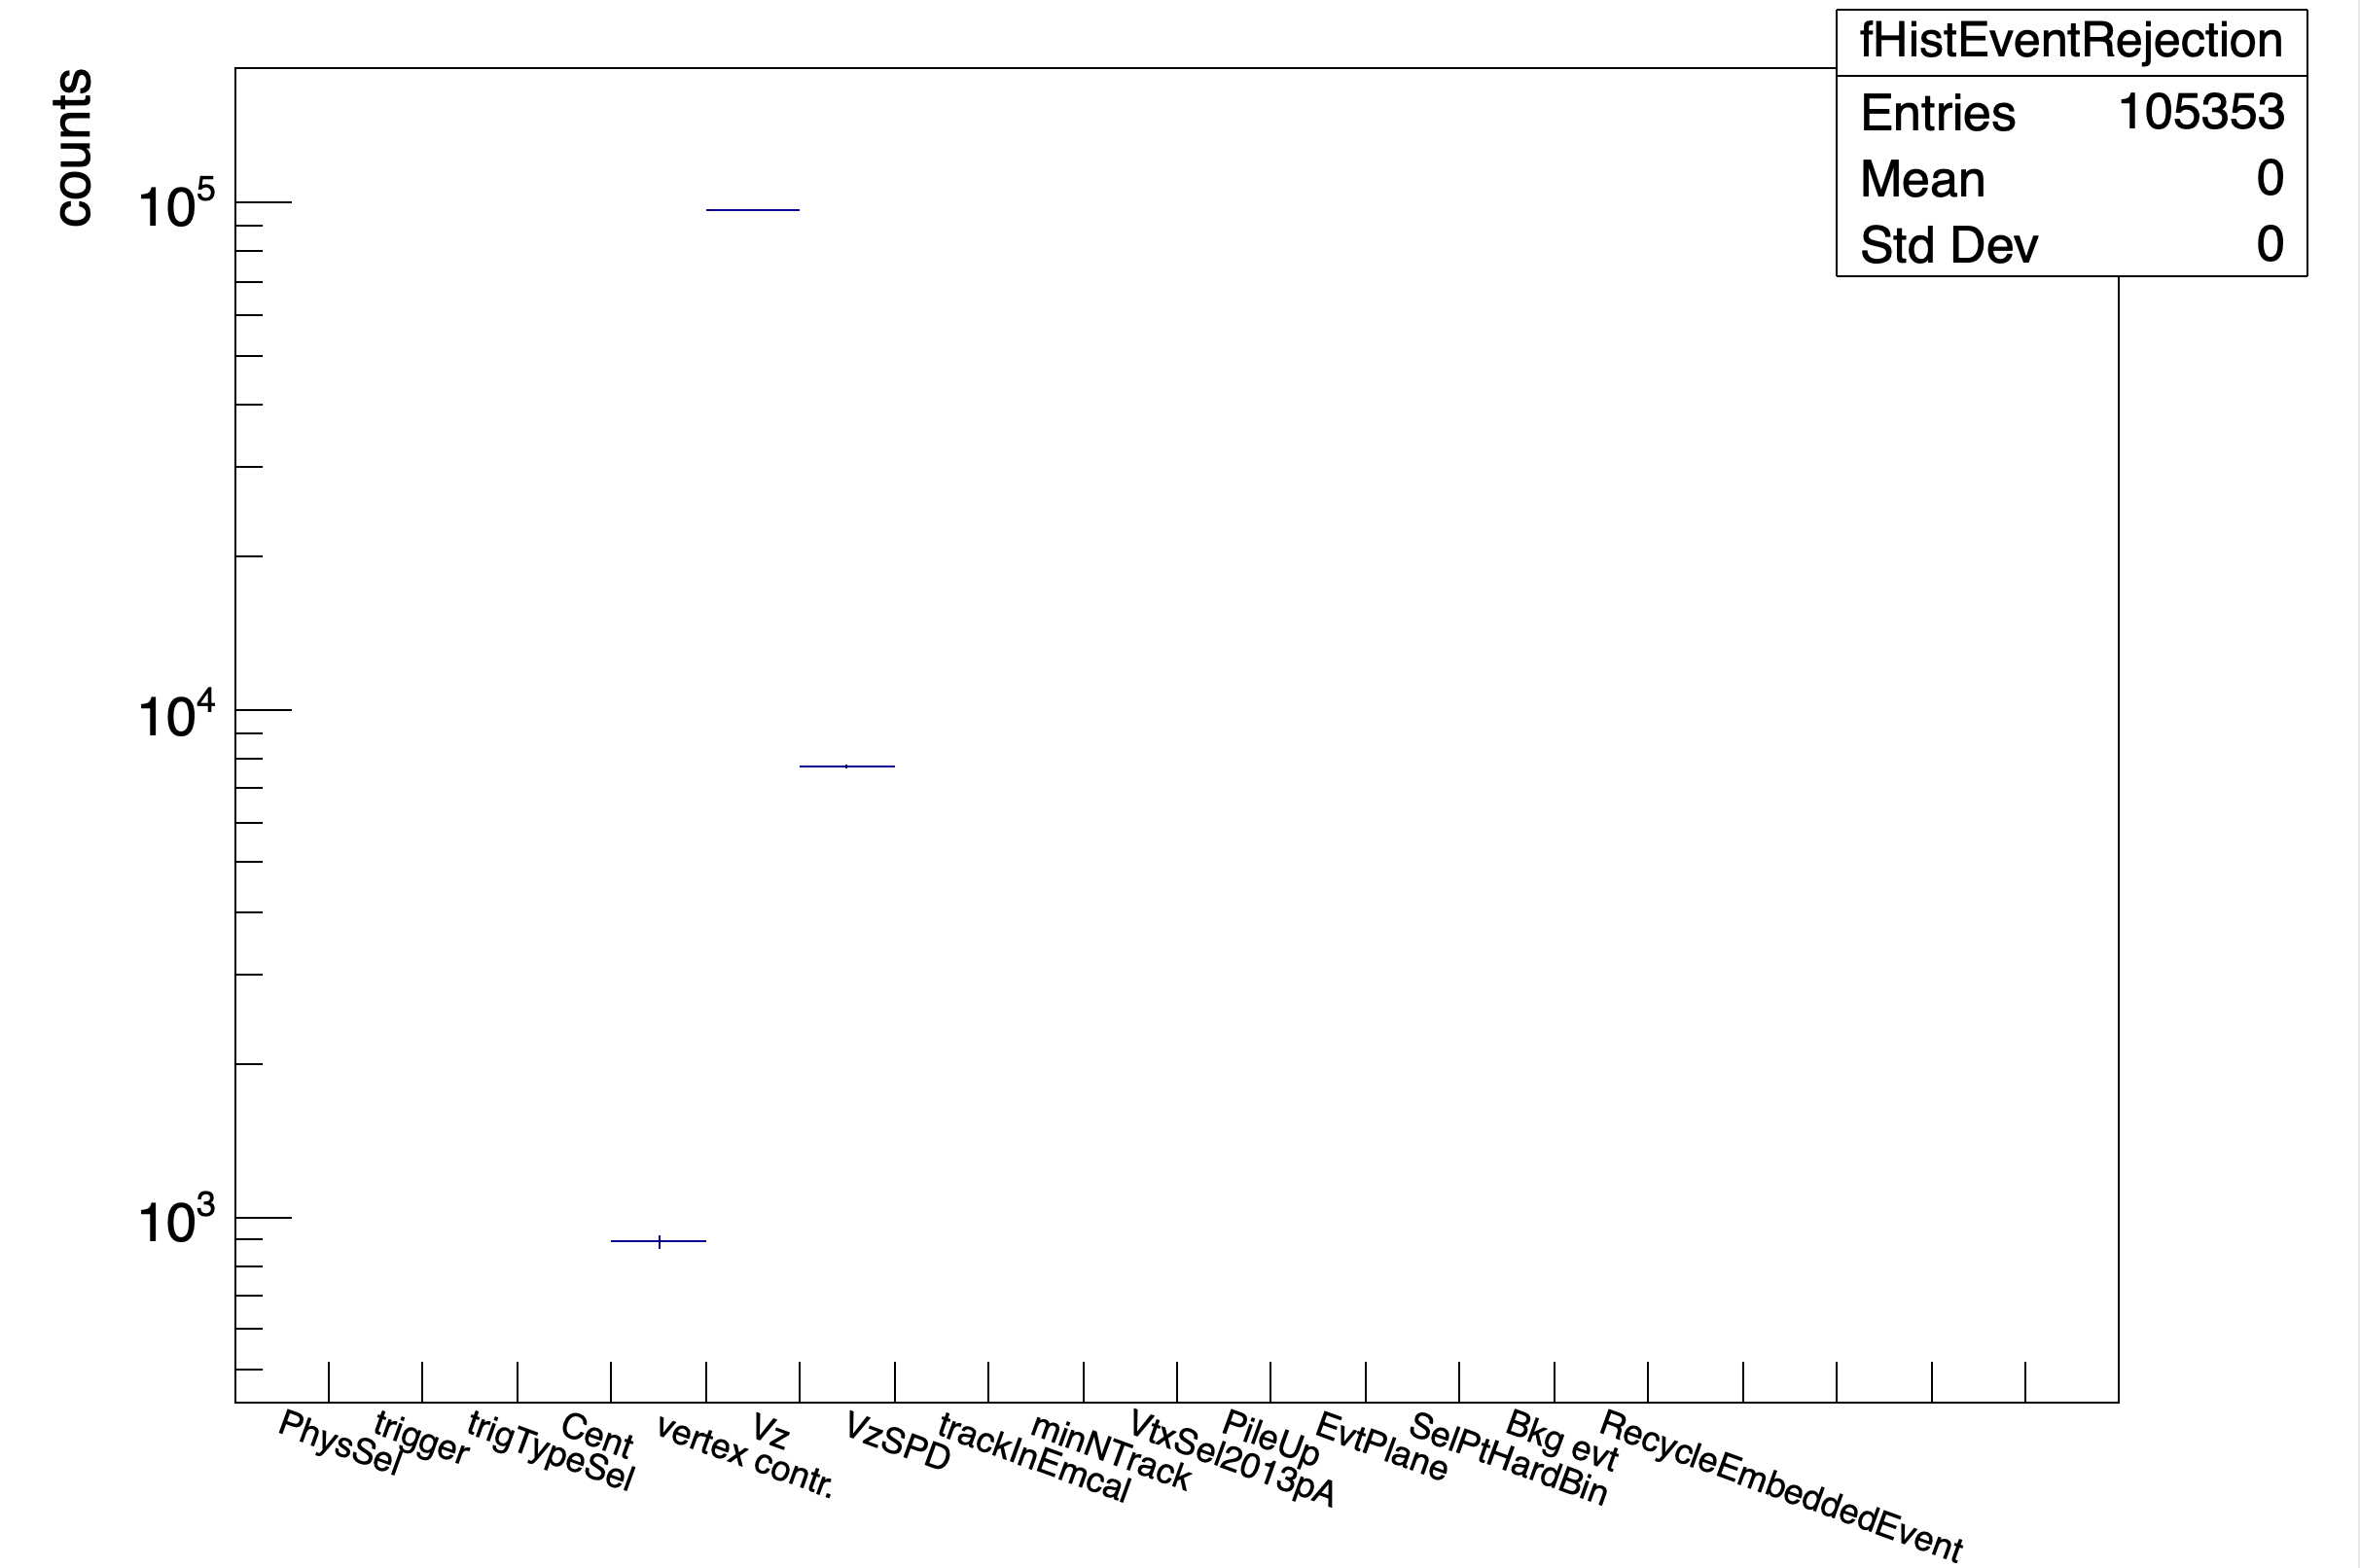
\includegraphics[width=\textwidth]{EventRejectionEGA}
    \caption{Emcal Triggered Event Rejection}
  \end{minipage}
\end{figure}